\section{【实现】slab算法的简化设计实现}\label{ux5b9eux73b0slabux7b97ux6cd5ux7684ux7b80ux5316ux8bbeux8ba1ux5b9eux73b0}

\subsection{数据结构描述}\label{ux6570ux636eux7ed3ux6784ux63cfux8ff0}

slab 算法采用了两层数据组织结构。在最高层是
slab\_cache,这是一个不同大小slab
缓存的链接列表数组。slab\_cache的每个数组元素都是一个管理和存储给定大小的空闲对象(obj)的slab
结构链表,这样每个slab设定一个要管理的给定大小的对象池,占用物理空间连续的1个或多个物理页。slab\_cache的每个数组元素管理两种slab列表:

\begin{itemize}
\tightlist
\item
  slabs\_full:完全分配的 slab
\item
  slabs\_notfull:部分分配的 slab
\end{itemize}

注意 slabs\_notfull列表中的 slab 是可以进行回收(reaping),使得slab
所使用的内存可被返回给操作系统供其他子系统使用。

slab 列表中的每个 slab
都是一个连续的内存块(一个或多个连续页),它们被划分成一个个obj。这些obj是中进行分配和释放的基本元素。由于对象是从
slab 中进行分配和释放的,因此单个 slab 可以在 slab
链表之间进行移动。例如,当一个 slab 中的所有对象都被使用完时,就从
slabs\_notfull 链表中移动到 slabs\_full 链表中。当一个 slab
完全被分配并且有对象被释放后,就从 slabs\_full 列表中移动到
slabs\_notfull列表中。下面是ucore中的slab架构图:

\begin{figure}[htbp]
\centering
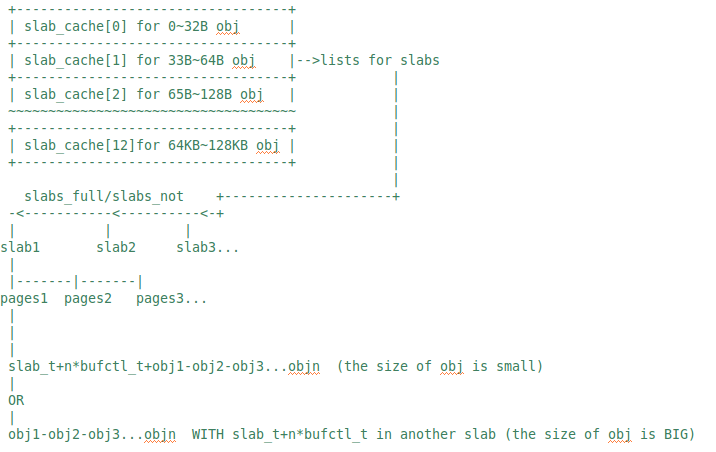
\includegraphics{figures/9.png}
\caption{8}
\end{figure}

slab架构图

\subsection{分配与释放内存实现描述}\label{ux5206ux914dux4e0eux91caux653eux5185ux5b58ux5b9eux73b0ux63cfux8ff0}

现在来看一下能够创建新 slab 缓存、向缓存中增加内存、销毁缓存的接口以及
slab 中对对象进行分配和释放操作的slab相关操作过程和函数。

第一个步骤是通过执行slab\_init函数初始化slab\_cache 缓存结构。然后其他
slab
缓存函数将使用该引用进行内存分配与释放等操作。ucore中最常用的内存管理函数是
kmalloc 和 kfree 函数。这两个函数的原型如下:

\begin{itemize}
\tightlist
\item
  void *kmalloc( size\_t size );
\item
  void kfree(void *objp );
\end{itemize}

在分配任意大小的空闲块时,kmalloc通过调用kmem\_cache\_alloc函数来遍历对应size的slab,来查找可以满足大小限制的缓存。如果kmem\_cache\_alloc函数发现slab中有空闲的obj,则分配这个对象;如果没有空闲的obj了,则调用kmem\_cache\_grow函数分配包含1到多页组成的空闲slab,然后继续分配。要使用
kfree
释放对象时,通过进一步调用kmem\_cache\_free把分配对象返回到slab中,并标记为空闲,建立空闲obj之间的链接关系。

\lstinline!(可进一步详细一些)!
